\documentclass[12pt]{article}

\usepackage{graphicx}
\usepackage{pdfpages}
\usepackage{listings}
\usepackage{amsmath}
\usepackage{amsfonts}
\usepackage{subcaption}
\usepackage{tikzsymbols}
\usepackage{algorithm}
\usepackage{algpseudocode}

% Redefinér til norsk tittel på figur og innholdfortegnelse, og algoritmekodeord
\renewcommand{\figurename}{Fig.}
\renewcommand{\contentsname}{Innhold}

\algrenewcommand\algorithmicwhile{\textbf{mens}}
\algrenewcommand\algorithmicdo{\textbf{gjør}}
\algrenewcommand\algorithmicend{\textbf{slutt}}
\algrenewcommand\algorithmicprocedure{\textbf{prosedyre}}
\makeatletter
\renewcommand{\ALG@name}{Algoritme}
\makeatother

% Endre font
% \usepackage[adobe-utopia]{mathptmx}
% \usepackage[T1]{fontenc}

\title{TTK4260 Innføring i Multivariat Datamodellering}
\date{}
\author{Kristian Løvland}

\begin{document}

\maketitle
\tableofcontents

\newpage
\section{Introduksjon}
Dette dokumentet er et forsøk på å skaffe meg en strukturert oversikt over et middels strukturert fag. Ting er først og fremst hentet fra slides, men også noe fra lærebøker jeg kanskje legger til som kilder senere.

\newpage
\section{Grunnleggende statistikk}
Til grunn for alle multivariate metoder som kommer senere, ligger den grunnleggende statistikken som forhåpentligvis er kjent fra før. Den oppsummeres her i korte trekk.

\subsection{Noen småting}
\subsubsection{Notasjon}
Gjennom denne oppsummeringen brukes følgende notasjon
\begin{itemize}
\item Skalare variabler og funksjoner skrives med små bokstaver -- $\alpha, x, g(\cdot)$
\item Vektorvariabler og -funksjoner skrives med små, fete bokstaver -- $\mathbf{\alpha}, \mathbf{x}, \mathbf{g(\cdot)}$. Eventuelt vanlige, små bokstaver som vist i forrige punkt. Jeg er litt slepphendt til tider.
\item Matriser skrives med store bokstaver -- $A, X$
\item Transponert, invers, pseudoinvers -- $\cdot^T, \cdot^{-1}, \cdot^\dagger$
\item Definisjonsmengder skrives med kaligrafiske bokstaver, eller stor theta -- $\mathcal{X}, \mathcal{Y}, \mathcal{D}$ eller $\Theta$
\end{itemize}

\subsubsection{Definisjoner}
En funksjon \(\phi(\boldsymbol{y}): \mathcal{Y}^{N} \mapsto \mathbb{R}^{M}\) er en \textbf{observator} dersom den er målbar, og den er uavhengig av $\theta$. En observator \(\phi(\boldsymbol{y}): \boldsymbol{y}^{N} \mapsto \Theta\) er en \textbf{estimator} dersom den er målbar og uavhengig av $\theta$ (dvs. den er en observator med verdimengde lik $\Theta$.

\subsubsection{Antagelser}
Når vi snakker om regresjon, antar vi at dataen $y_t$ genereres av funksjonen \(y_{t}=f\left(u_{t} ; \theta\right)+v_{t}\), og at dette resulterer i et datasett \(\mathcal{D}=\left\{\left(u_{t}, y_{t}\right)\right\}_{t=1, \ldots, N}\). Ved hjelp av parametre \(\theta \in \Theta\), hypoteserommet vårt, vil vi finne en estimator \(\widehat{\theta} \in \Theta\) som best mulig forklarer datasettet vårt.

Hva betyr det å "best mulig forklare $\mathcal{D}$? Det finnes det ulike tolkninger av.

\subsection{Minste kvadrater}
\label{sec:minste_kvadrater}
En naturlig tolkning av spørsmålet om å best mulig forklare datasettet vha $\theta$, er å finne parameteren som ved bruk av vår antatte modell $f(u_t; \theta)$, gir den korteste avstanden fra predikert datasett til faktisk datasett. "Avstand" har her den vanlige, euklidiske tolkningen, slik at en minste kvadraters estimator av en parameter $\theta$ gitt et datasett $\mathcal{D}$ og en modell $f(u_t; \theta)$, er gitt av
\begin{equation}
\widehat{\theta}_{\mathrm{LS}}=\arg \min _{\theta \in \Theta}\left\|\left[\begin{array}{c}
{y_{1}} \\
{\vdots} \\
{y_{N}}
\end{array}\right]-\left[\begin{array}{c}
{f\left(u_{1} ; \theta\right)} \\
{\vdots} \\
{f\left(u_{N} ; \theta\right)}
\end{array}\right]\right\|^{2}=\arg \min _{\theta \in \Theta} \sum_{t=1}^{N}\left(y_{t}-f\left(u_{t} ; \theta\right)\right)^{2}
\end{equation}
En nyttig verdi som følger av dette estimatet er residualen $r_{t}(\theta):=y_{t}-f\left(u_{t} ; \theta\right)$.

En nyttig klasse av problemer er de \textbf{separable} problemene. Disse er på formen
\begin{equation}
y_{t}=\sum_{j=1}^{n} \theta_{j} \phi_{j}\left(u_{t}\right)+e_{t}
\end{equation}
Dvs. at parameterne som skal estimeres inngår lineært i modellen vår. Da kan $\phi(u_t)$ være så komplisert den vil, LS-problemet vil uansett reduseres til et lineært likningssett på formen
\begin{equation}
\left[\begin{array}{c}
{y_{1}} \\
{\vdots} \\
{y_{N}}
\end{array}\right]=\left[\begin{array}{ccc}
{\phi_{1}\left(u_{1}\right)} & {\cdots} & {\phi_{n}\left(u_{1}\right)} \\
{\vdots} & {} & {\vdots} \\
{\phi_{1}\left(u_{N}\right)} & {\cdots} & {\phi_{n}\left(u_{N}\right)}
\end{array}\right]\left[\begin{array}{c}
{\theta_{1}} \\
{\vdots} \\
{\theta_{n}}
\end{array}\right]+\left[\begin{array}{c}
{e_{1}} \\
{\vdots} \\
{e_{N}}
\end{array}\right]
\end{equation}
Som mer kompakt kan skrives som
\begin{equation}
\boldsymbol{y}=\Phi(\boldsymbol{u}) \boldsymbol{\theta}+\boldsymbol{e}
\end{equation}
Målet vårt er å minimere $\mathbf{e}$. Dette kan gjøres vha. lineær programmering, men om vi ikke har begrensninger i $\theta$, dvs. $\Theta = \mathbb{R}^n$ for en eller annen $n$, kan dette løses eksplisitt som
\begin{equation}
\widehat{\theta}_{\mathrm{LS}}=\arg \min _{\boldsymbol{\theta} \in \mathbb{R}^{n}}\|\boldsymbol{y}-\Phi(\boldsymbol{u}) \boldsymbol{\theta}\|^{2}
\end{equation}
Ved å derivere dette og sette det lik null får vi \textbf{normallikningene}
\begin{equation}
\Phi(\boldsymbol{u})^{T} \Phi(\boldsymbol{u}) \widehat{\theta}_{\mathrm{LS}}=\Phi(\boldsymbol{u})^{T} \boldsymbol{y}
\end{equation}
Men hva om $
\Phi(\boldsymbol{u})^{T} \Phi(\boldsymbol{u})
$ ikke er invertibel? Da vil ikke normallikningene ha noen entydig løsning. Dette ordner vi ved å bruke \textbf{pseudoinversen}, som har noen kjekke egenskaper (nærmeste løsning hvis ingen løsning eksisterer, løsning med minst norm hvis mange løsninger eksisterer).

Noen ganger er imidlertid ikke alle tilstander like viktige. Dette løser vi ved å multiplisere hver feil med en vekt, slik at minimeringsproblemet (for ubegrensede problemer) blir
\begin{equation}
\widehat{\theta}_{\mathrm{WLS}}=\arg \min _{\boldsymbol{\theta} \in \mathbb{R}^{n}}(\boldsymbol{y}-\Phi(\boldsymbol{u}) \boldsymbol{\theta})^{T} W(\boldsymbol{y}-\Phi(\boldsymbol{u}) \boldsymbol{\theta})
\end{equation}
Mer kompakt kan dette skrives som $
=\arg \min _{\boldsymbol{\theta} \in \mathbb{R}^{n}}\|\boldsymbol{y}-\Phi(\boldsymbol{u}) \boldsymbol{\theta}\|_{W^{-1}}^{2}
$. Et nytt sett med normalligninger faller ut av dette, nå blir 
\begin{equation}
\Phi(\boldsymbol{u})^{T} W \Phi(\boldsymbol{u}) \boldsymbol{\theta}=\Phi(\boldsymbol{u})^{T} W \boldsymbol{y}
\end{equation}
som kan løses likt som tidligere, f.eks. med pseudoinvers.

Hva om problemet vårt er ulineært (ikke separabelt)? Optimeringsproblemet kan fortsatt være veldefinert, og da kan det løses numerisk. MATLAB gjør dette med \texttt{fmincon}, og de fleste programmeringsspråk med respekt for seg selv har rammeverk som gjør det samme.

\subsection{Maksimal sannsynlighet}
Forrige avsnitt ga en rent geometrisk tolkning av minste kvadrater. Ofte har min imidlertid kunnskap om de statistiske egenskapene til støyen og feilen som forsøpler dataen din, og denne informasjonen er gjerne nyttig å bruke. Utgangspunktet for dette er sannsynlighetsfordelingen, skrevet som $p(y ; \theta)$. Ofte operer man med $\theta$ fiksert og $y$ varierende. I vårt tilfelle er $y$ gitt (den utgjør datasettet vårt $\mathcal{D}$, og vi er ute etter å finne en $\theta$ som best forklarer dette. Da kalles $p(y ; \theta)$ for \textbf{sannsynlighet}.

Med dette definert er vi klare for å definere vår maksimale sannsynlighetsestimator
\begin{equation}
\widehat{\theta}_{\mathrm{ML}}=\arg \max _{\theta \in \Theta} p(\mathcal{D} ; \theta)
\end{equation}
Vi ser at denne ligner i formen på LS-estimatoren, men at funksjonen $p$ gir oss mer valgfrihet, og muligheter til å inkludere kjent informasjon om modell og data.

Det er verdt å merke seg at et ML-estimat ikke nødvendigvis trenger å eksistere. Man kan komme opp med massevis av eksempler på at denne ikke eksiterer, f.eks. kan man la $\Theta$ er en åpen mengde. Hvis $p$ er kontinuerlig og $\Theta$ er kompakt tror jeg imidlertid vi kan føle oss ganske trygge, i hvert fall hvis man er av typen som stoler på det Weierstrass hadde å si oss.

Et viktig eksempel på en ML-estimator er når $p$ er normalfordelt. Da vil sannsynlighetsfunksjonen til et datasett være gitt av
\begin{equation}
p\left(y_{1}, \ldots, y_{N} ; m, \sigma^{2}\right)=\prod_{t=1}^{N} p\left(y_{t} ; m, \sigma^{2}\right)=\prod_{t=1}^{N}\left(\frac{1}{\sqrt{2 \pi \sigma^{2}}} \exp \left(-\frac{1}{2} \frac{\left(y_{t}-m\right)^{2}}{\sigma^{2}}\right)\right)
\end{equation}
Dette grumsete uttrykket motiverer definisjonen av log-sannsynlighetsfunksjonen. Siden $\log(\cdot)$-funksjonen er monotont stigende i input-argumentet sitt, vil maksimerende input til funksjonen være lik maksimerende input til logaritmen av funksjonen. Vi definerer
\begin{equation}
\ell(\theta):=-\log p(\mathcal{D} ; \theta)
\end{equation}
I eksempelet med normalfordelt $p$ vil vi nå kunne formulere
\begin{equation}
\widehat{\theta}_{\mathrm{ML}}=\arg \max _{\theta \in \Theta} p(\mathcal{D} ; \theta) = \arg \min _{\theta \in \Theta} \ell(\theta)
\end{equation}
Eksponential- og logaritmefunksjonen spiller hverandre gode, og ved litt regning kan man se at
\begin{equation}
\arg \min _{m \in \mathbb{R}, \sigma^{2} \in \mathbb{R}_{+}} \ell\left(m, \sigma^{2}\right)=\arg \min _{m \in \mathbb{R}, \sigma^{2} \in \mathbb{R}_{+}} N \log \left(\sigma^{2}\right)+\frac{\sum_{t=1}^{N}\left(y_{t}-m\right)^{2}}{\sigma^{2}}
\end{equation}
Dennes gradient settes lik null, men her vil det inngå informasjon vi ikke har tilgang på. Vi ender opp med å benytte estimatene, og får
\begin{equation}
\bar{m}=\frac{1}{N} \sum_{t=1}^{N} y_{t}
\end{equation}
\begin{equation}
\bar{\sigma}^{2}=\frac{1}{N} \sum_{t=1}^{N}\left(y_{t}-\bar{m}\right)^{2}
\end{equation}
som ser fornuftig ut.
\subsection{Maksimal a posteriori}
Vi begynner med Bayes' lov
\begin{equation}
P(A | B)=\frac{P(A B)}{P(B)} = \frac{P(B | A) P(A)}{P(B)}
\end{equation}
som kan bevises ved Venn-diagram eller lignende.

Ved å bytte ut $A$ og $B$ med $\theta$ og $y$, får vi en måte å oppdatere vår tro om en variabel sin fordeling på, basert på data. Vi er imidlertid avhengige av å ha en initiell formening om fordelingen til $\theta$, dette kalles en \textbf{prior}. I praksis vil denne gjerne gjøre få antagelser, men utelukke fullstendig urealistiske muligheter (f.eks. utelukke negativ høyde på personer, om man vil estimere dette). Med en modell $P(y | \theta)$, en prior $P(\theta)$, og data som gir oss $P(y)$, får vi da
\begin{equation}
P(\theta | y)=\frac{P(y | \theta) P(\theta)}{P(y)}
\end{equation}
Basert på denne nye, evidensbaserte fordelingen, kan vi definere estimatoren
\begin{equation}
\widehat{\theta}_{\mathrm{MAP}}:=\arg \max _{\theta \in \Theta} P(\theta | y)=\arg \max _{\theta \in \Theta} \frac{P(y | \theta) P(\theta)}{P(y)}=\arg \max _{\theta \in \Theta} P(y | \theta) P(\theta)
\end{equation}
som vil være moden til den posteriore fordeling. Merk at denne ikke trenger å være representativ for fordelingen, f.eks. hvis fordelingen har en smal, høy topp langt unna "tyngdepunktet".
\subsection{Statistiske ytelsesindekser}
Vi går kort gjennom noen statistiske ytelsesindekser (dvs. for ytelsen til en estimator) for tre ulike typer problemstilling.

\subsubsection{Regresjonsproblemer}
En mye brukt indeks er \textbf{Mean Squared Error (MSE)}
\begin{equation}
\textrm{MSE} = \mathbb{E}\left[\|\theta-\widehat{\theta}\|^{2}\right]
\end{equation}
Av denne følger \textbf{Root Mean Square Error}
\begin{equation}
\textrm{RMSE} = \sqrt{\mathbb{E}\left[\|\theta-\widehat{\theta}\|^{2}\right]}
\end{equation}
Det er viktig å merke seg at siden MSE er en funksjon av $\theta$, så kan den ikke regnes ut. Hvorfor bryr vi oss om den da? Tja, den kan i hvert fall inspirere lignende indekser. \textbf{Residual Sum of Squares (RSS)} baserer seg på residualene til estimatene
\begin{equation}
\operatorname{RSS}(\widehat{\theta}):=\sum_{i}\left(y_{i}-\widehat{y}_{i}(\widehat{\theta})\right)^{2}
\end{equation}
Det finnes imidlertid problemer med alle disse. Først og fremst er det et problem at de er avhengig av mengden av og størrelsen på dataen man vurderer estimatene av. Man vektlegger å unngå avvik i estimatene fra store målinger mer enn små. En metode som fungerer noe bedre, uten å bruke normalisering, er å bruke 1-normen i stedet for kvadratet. Dette gjøres i \textbf{Mean Absolute Deviaton (MAD)}
\begin{equation}
\mathrm{MAD}:=\mathbb{E}[|y-\widehat{y}|]
\end{equation}
En metode som bruker en form for normalisering er \textbf{Fraction of Variance Unexplained (FVU)}
\begin{equation}
\mathrm{FVU}(\widehat{\theta}):=\frac{\operatorname{RSS}(\widehat{\theta})}{\operatorname{var}(y)}=\frac{\sum_{i}\left(y_{i}-\widehat{y}_{i}(\widehat{\theta})\right)^{2}}{\sum_{i}\left(y_{i}-\frac{1}{N} \sum_{i} y_{i}\right)^{2}}
\end{equation}
Denne må tolkes med måte, siden hva som er en god forklaringgrad er veldig avhengig av hva slags felt man jobber i, og det konkrete bruksområdet. Dette er uansett en mye brukt indeks, men da i form av $R^{2}$
Denne tolkes som "andel av variansen i avhengig variable som er predikerbar fra de uavhengige variablene".

\subsubsection{Klassifiseringsproblemer}
Vi diskuterer her klassifisering i form av "ja/nei". Da kan man gjøre to typer feil: Falsk positiv (\textbf{Type 1}) og falsk negativ (\textbf{Type 2}). Det finnes mange mer eller mindre naturlige måter å vurdere om en estimator sine ja/nei-svar er gode på:

\begin{itemize}
\item \textbf{Prevalens} -- Hvor ofte opptrer ja-tilfellet i datasettet vårt?
\item \textbf{Nøyaktighet} -- Hvor ofte har klassifikatoren rett?
\item \textbf{Feilklassifiseringsrate} -- Hvor ofte tar klassifikatoren feil?
\item \textbf{Presisjon} -- Når klassifikatoren gjetter ja, hvor ofte er dette rett?
\item \textbf{Falsk positiv-rate} -- Når svaret er nei, hvor ofte gjetter klassifikatoren ja?
\item \textbf{Sensitivitet} -- Når svaret er ja, hvor ofte gjetter klassifikatoren ja?
\item \textbf{Spesifitet} -- Når svaret er nei, hvor ofter gjetter klassifikatoren nei?
\end{itemize}

Man kan også kombinere to av disse for å få \textbf{F1-score}
\begin{equation}
\textrm{F1-score} = 2 \frac{\textrm{presisjon} \cdot \textrm{
sensitivitet}}{\textrm{presisjon} + \textrm{
sensitivitet}}
\end{equation}

\subsubsection{Sammenligning av sannsynlighetsfordelinger}
I utledning av ulike former for estimatorer eller ytelsesindekser ønsker man gjerne å basere seg på statistisk teori enn å bruke ``sunn fornuft''. Et mye brukt mål på likheten mellom to sannsynlighetsfordelinger er \textbf{Kullback-Leibler-divergens}. Denne er utledet med utgangspunkt i informasjonsteori. Gitt sannsynlighetsfordelinger $p_0$ og $p_n$ og data $\mathcal{D}$, forteller KL-divergensen hvor mye informasjon som tapes på å representere $p_0$ med $p_n$ (dette er ikke symmetrisk), og kan dermed brukes som mål på hvor ``forskjellige'' fordelingene er. Den er gitt av
\begin{equation}
		K L\left(p_{0}, p_{n}\right):=\int \log \left(\frac{p_{0}\left({\mathcal{D}}, \theta_{0}\right)}{p_{n}\left({\mathcal{D}}, \theta_{n}\right)}\right) p_{0}\left({\mathcal{D}}, \theta_{0}\right) d {\mathcal{D}}
\end{equation}


\subsection{Bias vs. varians}
Dette er en avveining man ikke slipper unna når man bedriver estimering. La oss bruke MSE for å illustrere dette. Anta at vi estimerer en parameter $\theta$ med $\hat{\theta}$. La 

\begin{equation}
\begin{array}{l}{\mathcal{V}:=\widehat{\theta}-\mathbb{E}[\widehat{\theta}]} \\ {\mathcal{B}:=\mathbb{E}[\widehat{\theta}]-\theta}\end{array}
\end{equation}
Da er
\begin{align}
\mathbb{E}\left[\|\hat{\theta}-\theta\|^{2}\right] &=\mathbb{E}\left[\|\widehat{\theta}-\mathbb{E}[\widehat{\theta}]+\mathbb{E}[\widehat{\theta}]-\theta\|^{2}\right] \\ \nonumber
&=\mathbb{E}\left[\|\mathcal{V}+\mathcal{B}\|^{2}\right]\\ \nonumber
&=\mathbb{E}\left[(\mathcal{V}+\mathcal{B})^{T}(\mathcal{V}+\mathcal{B})\right] \\ \nonumber
&=\mathbb{E}\left[\|\mathcal{V}\|^{2}+\|\mathcal{B}\|^{2}+2 \mathcal{V}^{T} \mathcal{B}\right] \\ \nonumber
&=\mathbb{E}\left[\|\mathcal{V}\|^{2}\right]+\|\mathcal{B}\|^{2}
\end{align}
Dvs. at en estimator sin forventede feil vil bestå både av et bias-ledd (systematisk feil) og et varians-ledd. For å oppnå et godt estimat må begge disse minimeres, men å minimere bias og varians er typisk motstridende interesser, og man må gjøre vurderinger av datasett og estimeringsmetodikk for å finne en god avveining.

Denne avveiningen henger sammen med hvor komplisert man gjør forklaringsmodellen $f(u_t; \theta)$. Om man gjør den veldig komplisert vil man kunne følge dataen nøyaktig, men man vil være utsatt for at dette ikke lar seg generalisere til andre datasett \textbf{overfitting}. Dette svarer til lav bias, men stor varians. Om modellen er for enkel vil man få en enkel modell som generaliserer, men man vil også kunne unngå å beskrive viktig struktur i dataen. Dette er \textbf{underfitting}, og svarer til liten varians, men stor bias.

Det finnes verktøy som kan brukes som hjelp til å ta beslutninger om slike ting, som vi kommer tilbake til senere.

\section{Multivariat Dataanalyse}
Her begynner de nye metodene. Jeg ser frem til å lære ny teori, og på å anvende denne \Cooley.
 
\subsection{Eksperimentdesign}
\textbf{Eksperimentdesign} er forhåndsplanlagt, systematisk variasjon av kontrollerte faktorer i et eksperiment, med det formål å få mest mulig informasjon med minst mulig innsats. Dette er et alternativ til den naive måten å gjøre det på, dvs. å endre én variabel om gangen. Denne måten å gjøre det på har flere fordeler. I tillegg til den åpenbare fordelen med et lavt, forutsigbart antall eksperimenter som må gjennomføres, får man mer informasjon om interaksjon mellom variabler. Det finnes flere ulike typer eksperimentdesign. Her går vi gjennom noen av dem.

\subsubsection{Factorial designs}
Dette er den enkleste metoden som gås gjennom. Den er optimal for å detektere hovedeffekter, og deres interaksjoner. Den er også basisen for mange andre ttyper eksperimentdesign. Her velger man seg to verdier for hver input-variabel, og gjennomfører et eksperiment for hver av de mulige kombinasjonene av disse. Altså trenger man $2^n$ eksperimenter når man har $n$ variable. La $y_+$ og $y_-$ være observasjonene av en variabel $y$ i de to ulike tilstandene, og $n$ være antall observasjoner for hver av disse. Effekten av endringene i $y$ er da gitt av

\begin{equation}
	\Delta y = \frac{\sum y_+} {n_+} - \frac{\sum y_-}{n_-}
\end{equation}

Før man begynner å gjennomføre et eksperiment, er det viktig å regne ut 
den statistiske styrken til eksperimentet. Denne er avhengig av

\begin{enumerate}
	\item $\delta$: Hva som regnes som en signifikant endring 
	\item $\sigma$: Støy i målt responsvariabel
	\item Antall eksperimenter
	\item $\alpha$: Signifikansnivå
\end{enumerate}

Basert på disse parameterne kan man regne ut

\begin{equation}
	\textrm{Statistisk styrke} = (1 - \beta) \cdot 100 \%
\end{equation}

Denne kan tolkes som sannsynligheten for å ``avsløre'' en effekt av størrelsedelta, gitt støyet som nevnt over. Dette er en signal til støy-ratio, gitt av$\frac{\Delta}{\sigma}$. Denne burde være høy, minst 80\%. I tillegg til å gjennomføre eksperimentene som nevnt over, kan det være nyttig å gjennomføre noen ekstra eksperimenter der tilstandene befinner seg rundt middelverdi, for å kunne estimere feilvarians. Repliserte eksperimenter er heller aldri noen ulempe å gjennomføre.

\subsubsection{Multippel lineær regresjon (MLR)}
En mer fornuftig (synes jeg) måte å analysere multivariabel data på er å sette opp en enkel lineær modell

\begin{equation}
	y = b_0 + b_1 x_1 + b_2 x_2 + \cdots + b_k x_k + f
\end{equation}

Den beste tilpasningen av en slik modell får man ved å minimere summen av kvadratavviket mellom modellprediksjon og faktisk data, som forklart i avsnitt \ref{sec:minste_kvadrater}. Når dette er gjennomført analyserers resultatene ved hjelp av en ANOVA-tabell (analysis of variance). I denne deles data inn i bidrag fra hhv. struktur og støy, slik at kvadratsummen

\begin{equation}
	SS_{total} = SS_{model} + SS_{error}
\end{equation}

Gitt $k$ forklaringsvariable og $l$ forsøk, vil ANOVA-tabellen for hele modellen se ut som i tabell \ref{tab:anova} (her betyr MS mean square). F-verdien er et mål på statistisk signifikans, og deler navn med fordelingen den er basert på. Denne observatoren oppfyller $E[F] = 1 + n \frac{\sigma_{model}^2}{\sigma_{error}^2}$, og en F-verdi langt over 1 gir dermed grunnlag for å forkaste nullhypotesen om at modellen vår ikke forklarer resultatene. 

\begin{table}[h]
	\centering
	\begin{tabular}{c|c|c|c||c|c}
		\textbf{Kilde} & \textbf{SS} & \textbf{df} & \textbf{MS} & \textbf{F-ratio} & \textbf{p-verdi} \\ \hline 
		Modell & $SS_{modell}$ & $k$ & $MSR = SS_{modell}/(k)$ & MSR/MSE & p \\
		Feil & $SS_{feil}$ & $l-k-1$ & $MSE = SS_{feil}/(l-k-1)$ & & \\
		Total & $SS_{total}$ & $l-1$ & $MST = SS_{total}/(l-1)$ & & 
	\end{tabular}
	\caption{ANOVA-tabellstruktur}
	\label{tab:anova}
\end{table}

Man kan også sette opp en ANOVA-tabell for enkeltledd i modellen, hver av disse vil ha samme struktur som øverste rad i tabelll \ref{fig:anova}.

\subsubsection{Fractional Factorial Designs}
Jeg vet ikke hva dette heter på norsk.

Full Factorial designs er kostbare hvis det er mange variabler. I Fractional Factorial designs gjennomfører man kun en delmengde av disse, og forsøker å dekke så ``mye'' som mulig av designrommet. Prisen man betaler er at estimatene av alle variablene ikke lenger kan være uavhengige.

For eksempel, gitt tre designvariabler $A$, $B$, $C$. Ved å velge å kun gjennomføre eksperimenter i planet $C = AB$, kan man halvere antall eksperimenter som gjennomføres.

\subsubsection{Optimeringsbaserte design}
Om man vet mer om hva slags respons man forventer i modellen sin, kan man utnytte denne informasjonen til eksperimentdesign. Det finnes mange metoder som baserer seg på ulike optimalitetskriterier. I pensum trekkes \textbf{Central Composite Design} og \textbf{Bob-Behnken Designs}, frem som viktige metoder. Begge er eksempler på bruk av \textbf{Response Surface Methodology}. Om man kjenner til begrensninger i tilstandsrommet kan man bruke dette til å utelukke umulige tilstander fra eksperiemntdesignet.

Uansett hvordan man velger å gjennomføre eksperimentene, bør man plotte fornuftige plott når man er ferdig. Dette gjelder stort sett alltid, har jeg inntrykk av.



\subsection{PCA}
Prinsipalkomponentanalyse (PCA) er en veldig nyttig metode som benyttes til bl.a. mønstergjenkjenning, dimensjonalitetsreduksjon, klyngeanalyse, klassifisering og utliggerdeteksjon. Den baserer seg på noen viktige konsepter fra lineæralgebra.

\subsubsection{Matematisk bakgrunn}

La vektorene $\mathbf{x}, \mathbf{y} \in V$, der $V$ er et indreprouktrom. Disse vektorene er \textbf{ortogonale} dersom indreproduktet $\langle \mathbf{x}, \mathbf{y} \rangle = 0$. To underrom $A$ og $B$ er ortogonale dersom alle vektorer i $A$ er ortogonal med alle vektorer i $B$, og omvendt. En mengde vektorer $S$ er ortonormal dersom alle vektorene den inneholder er ortogonale med hverandre, og har norm 1.

\textbf{Projeksjonen} av vektoren $\mathbf{y}$ på $\mathbf{x}$ er gitt av

\begin{equation}
\textrm{Proj}_{\mathbf{x}} \mathbf{y} = \frac{\langle \mathbf{x}, \mathbf{y} \rangle}{|\mathbf{x}|^2}\mathbf{x}
	\label{eq_projection}
\end{equation}

En matrise $A$ kan sees på som en \textbf{lineærtransformasjon}, f.eks. en rotasjon eller en skalering i en viss retning.

\subsubsection{Tolkning av PCA}
PCA går kort oppsummert ut på å finne vektorer som best mulig forklarer varians i dataen, og som er ortogonale med hverandre. Håpet er at noen få av disse \textbf{prinsipale komponentene} forklarer en stor del av variansen. Metoden har en fin geometrisk tolkning. La $S$ være en sirkel, og $A$ være en lineærtransformasjon (f.eks. representert av en matrise). Da vil $A$ (med mindre den er singulær) ha egenvektorer $\mathbf{v}_1$ og $\mathbf{v}_2$. Disse vil da strekkes med faktorene $\sigma_i$, egenverdiene deres. Dette er vist i figur \ref{fig:pca_skvis}.

\begin{figure}[h]
	\centering
	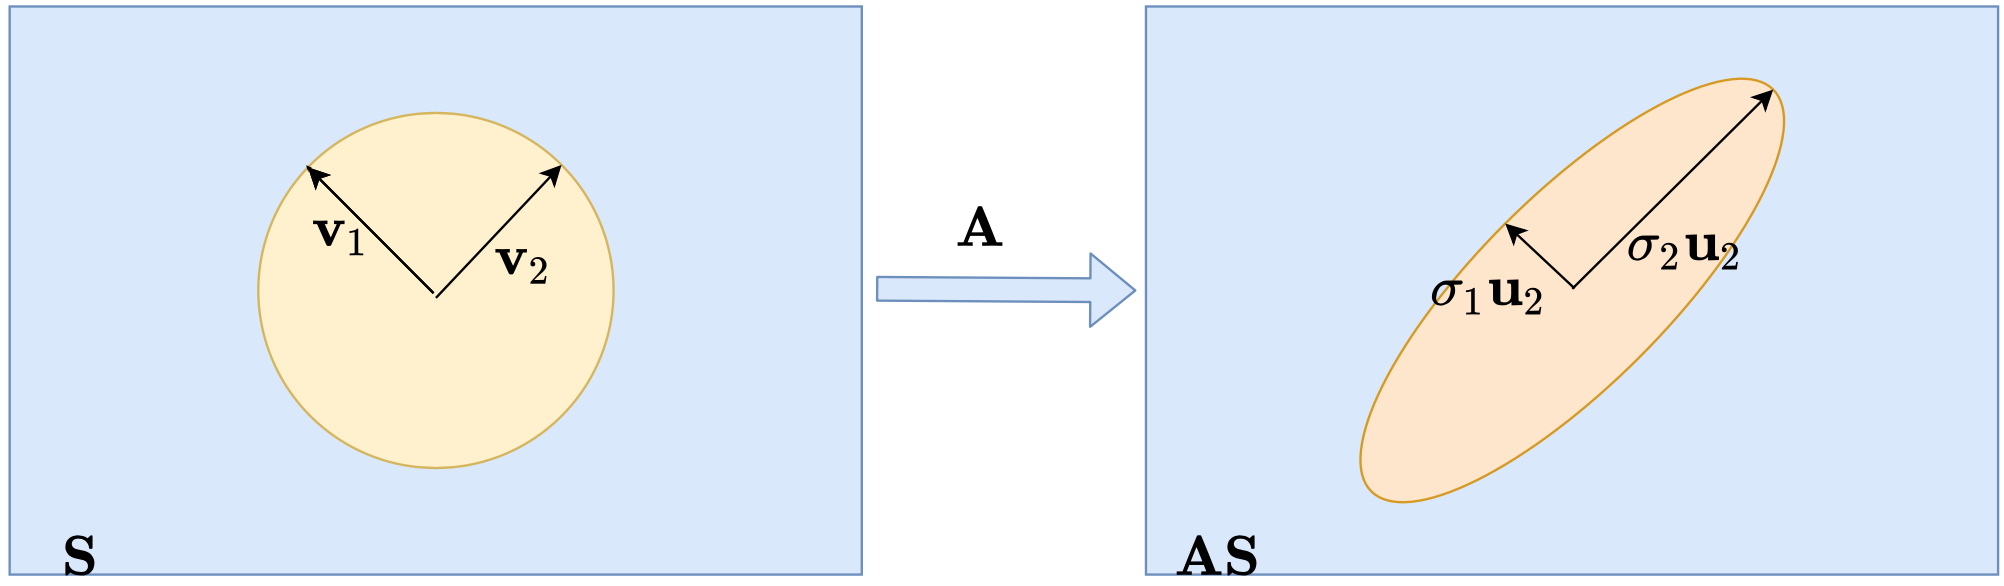
\includegraphics[width=\textwidth]{figurer/pca_skvis}
	\caption{Geometrisk tolkning av lineærtransformasjon}
	\label{fig:pca_skvis}
\end{figure}

For egenvektorer $\mathbf{v}_i$ med egenverdier $\sigma_i$ vil dermed

\begin{equation}
	A \mathbf{v}_j = \sigma_j \mathbf{u}_j
\end{equation}

For høyere dimensjon enn 2 (som i figuren) vil likningene være helt like. En hypersfære $\mathbf{V}$ av egenverdier transformeres av $A$ til en hyperellipse $\mathbf{U}$ under likningen

\begin{equation}
	A \mathbf{V} =\mathbf{U} \mathbf{\Sigma}
\end{equation}

Hvis egenvektorene til $A$ er lineært uavhengige, vil $\mathbf{V}$ være invertibel, og vi kan definere \textbf{singulærverdidekomposisjonen}

\begin{equation}
	A  =\mathbf{U} \mathbf{\Sigma} \mathbf{V}^*
\end{equation}

Ved å slå sammen matrisene $\mathbf{U} \mathbf{\Sigma}$ står vi igjen med en ny tolkning av $A$, forklart av kolonnene i $\mathbf{V}^*$ og kolonnene i $\mathbf{U} \mathbf{\Sigma}$. Dette er illustrert i figur \ref{fig:pca_komponentvis}. Mye av styrken til PCA ligger i at hvis $A$ har en lav nok underliggende dimensjon, kan vi approksimere $A$ ganske bra ved å kaste bort vektorene som svarer til lave singulærverdier $\sigma_i$. Modellordenen reduseres drastisk uten at vi mister viktig informasjon \Cooley.

\begin{figure}[h]
	\centering
	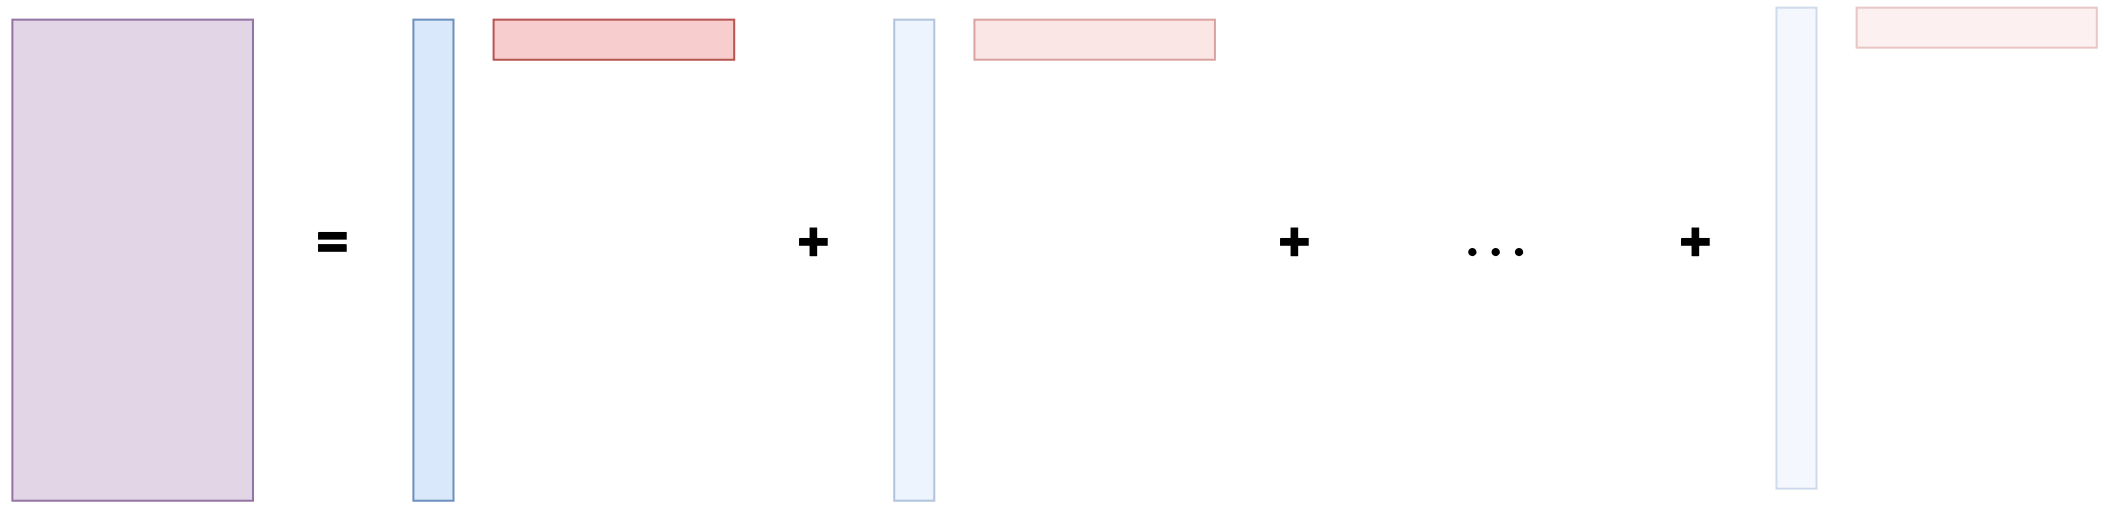
\includegraphics[width=\textwidth]{figurer/pca_komponentvis}
	\caption{Tolkning av SVD}
	\label{fig:pca_komponentvis}
\end{figure}

\subsubsection{Utledning av prinsipale komponenter}
Det finnes flere måter å finne de prinsipale komponentene. En av dem, kalt \textbf{egenverdidekomposisjonen}, baserer seg på at vi ønsker å maksimere variansen i ladningene $\mathbf{t} = \mathbf{Xp}$, der $X$ er dataen vår er $p$ er en prinsipal komponent (slik at $\mathbf{t}_j = \textrm{proj}_{\mathbf{p}} \mathbf{X}$, stol på dette). For å finne $p_1$, kan vi dermed løse optimeringsproblemet

\begin{equation}
	\max (\phi)=\boldsymbol{p}_{1}^{T} \boldsymbol{X}^{T} \boldsymbol{X} \boldsymbol{p}_{1}-\lambda\left(\boldsymbol{p}_{1}^{T} \boldsymbol{p}_{1}-1\right)
\end{equation}

som er funnet ved å inkludere begrensningen $\mathbf{p}_1^T \mathbf{p} = 1$ som Lagrange-multiplikator. Ved å derivere mhp. $\mathbf{p}_1$ og sette lik null, finner man at løsningen er gitt av likningen

\begin{equation}
	\mathbf{X}^T \mathbf{X} \mathbf{p}_1 = \lambda_1 \mathbf{p}_1
\end{equation}

Ved å innføre begrensningen $\mathbf{p}_1 \perp \mathbf{p}_2$ kan man finne at $\mathbf{p}_2$ kan finnes på akkurat tilsvarende vis osv. for de neste prinsipale komponentene.

PCA kan også gjøres ved å finne SVD-en til $X$, dette finnes det funksjoner for i de fleste \texttt{programmeringsspråk} som brukes til dataanalyse. Når man kjenner denne er dekomposisjonen av $\mathbf{X}$ i ladninger $\mathbf{p}_i$ med tilhørende score $\mathbf{t}_i$ gitt av

\begin{equation}
	\mathbf{X} = \mathbf{t}_1 \mathbf{p}_1^T + \mathbf{t}_2 \mathbf{p}_2^T + \cdots + \mathbf{E} = \sigma_1 \mathbf{u}_1 \mathbf{v}_1^T +  \sigma_2 \mathbf{u}_2 \mathbf{v}_2^T + \mathbf{E} 
\end{equation}


\subsubsection{NIPALS-algoritmen}
En effektiv metode for utregning av PC-er kalles Nonlinear Iterative Partial Least Squares (\textbf{NIPALS}). Denne ble blant annet brukt i tidlige versjoner av Google sin PageRank-algoritme. Algoritmen går ut på å iterativt finne hver prinsipale komponent, og å fjerne variabiliteten denne bidrar med før neste PC regnes ut. Noen fordeler med NIPALS er at man kan håndtere store datamengder i $\mathbf{X}$, at man kan håndtere manglende data, og at man er garantert konvergens. Pseudokoden under viser algoritmen. Merk at projeksjon av en matrise $X$ på en vektor $t$ etterfulgt av en normalisering mer kompakt kan skrives som 
\begin{equation}\frac{\textrm{proj}_t(X)}{|| \textrm{proj}_t(X) ||_2} = \frac{X^T t / t^T t}{|| X^T t / t^T t ||_2} = \frac{X^T t / t^T t}{\sqrt{(X^T t)^T (X^T t) / (t^T t)^2}} = \frac{X^T t}{|| X^T t ||_2}
\label{eq:normalisering_triks}
\end{equation}
Hovedideen bak NIPALS er å utlede ytreproduktene $t_i p_i^T$ én og én, med høyeste varians først. Disse vektorene finnes ved å iterativt tilpasse $p$ til $t$ vha. $X$, $t$ til $p$ vha. $X$, frem og tilbake helt til resultatet stabiliserer seg (dette kalles gjerne ``criss-cross regressions''). Pseudokode for NIPALS er som følger (merk at man antar at $X$ allerede er sentrert).

\begin{algorithm}
	\caption{NIPALS for PCA}\label{alg:nipals_pca} \begin{algorithmic}[1] \Procedure{NIPALS}{$X, n_\textrm{PCA}, t_\textrm{tol}$}\Comment{Numerisk utregning av PCA}
	\State $i \gets 1$
	\While{$i < n_\textrm{PCA}$}
	\State Initialisér $t_i$ (tilfeldig, eller som en av kolonnene i $X$)
	\While{Endring i $t_i > t_\textrm{tol}$}
	\State $p_i \gets \frac{X^T t_i}{|| X^T t_i ||_2}$ \Comment{Projeksjon av $X$ på $t_i$}
	\State $t_i \gets X p_i$ \Comment{Projeksjon av $X$ på $p_i$}
	\EndWhile
	\State $X \gets X - t_i p_i^T$ \Comment {Deflasjon}
	\State $i \gets i + 1$
	\EndWhile
\EndProcedure
\end{algorithmic}
\end{algorithm}

%\begin{algorithm}
%	\caption{NIPALS for PCA}
%	\label{alg:NIPALS_PCA}
%	\begin{algorithmic[1]}
%		\Procedure{NIPALS}{$X$}
%		\State Sentrér $X$-matrisen
%		\EndProcedure
%	\end{algorithmic}
%\end{algorithm}

\subsubsection{Visualisering av PCA}
Det finnes mange nyttige måter å bruke PCA på for å visualisere data. Kanskje blir dette kapitlet lengre etter hvert.


\subsection{Valg av modellorden, og validering}
I forrige delkapittel lovpriste vi PCA-ens evne til å reduserte dimensjonen til en datamatrise uten at vi mister informasjon. Men hvor mye kan man egentlig redusere denne dimensjonen, og hvordan velger man hvilken informasjon man har råd til å kaste vekk? Det er denne typen problemstilling \textbf{modellordenseleksjon} handler om.

\subsubsection{Problemformulering}
Modellordenseleksjon er et problem i mengden av \textbf{modellseleksjonsproblemer}. Disse går ut på å velge en statistisk modell av flere gitt et datasett som skal forklares. Dette kan virke enkelt (bare velg modellen som gir lavest kvadratavvik for datasettet da vel!), men få datasett representerer virkeligheten 100\%. Bias vs. varians-tradeoffen gjør seg dessverre gjeldende og tvinger oss til å balansere på en knivsegg mellom over- og undertilpassing av modellen vår. Uff.

\subsubsection{Motivasjon}
Anta at vi har et datasett med én observasjon, $y \sim \mathcal{N}(\mu, \sigma^2)$, som estimeres vha. funksjonen $\hat{\mu} (y)$. Hvordan vet vi hvor god denne stimatoren er? Vi kan jo forsøke å finne MSE av estimatoren direkte, det er bare ett problem (her har jeg vært litt lat med å vise utregninger):

\begin{equation}
\mathbb{E} [(\mu - \hat{\mu})^2] = \cdots = -n \sigma^2 + \mathbb{E} [(y - \mu)^2] + \underbrace{2 \textrm{cov}(y, \mu)}_{\textrm{trøbbel}}
\end{equation}

Det siste leddet har man vanligvis ikke kjennskap til. Hvordan kan vi da anslå hvor god en estimator er, når man ikke er så heldig å ha fått utdelt et testsett å teste på?

\subsubsection{Kryssvalidering}
Om man ikke har et dedikert testsett å validere en modell på, kan man lage sitt eget ved å dele opp treningssettet. Dette kalles \textbf{kryssvalidering}. Ulike måter å dele opp på gir ulike former for kryssvalidering.

Det er ønskelig å ha et så stort treningssett som mulig, så et naturlig valg vil være å kun utelate én observasjon som treningssett. Ved å utelate en og en observasjon, kan man regne ut $n$ ulike MSE-er. Gjennomsnittet av disse gir \textbf{Leave One Out Cross-Validation (LOOCV)}.

Å tilpasse en modell $n$ ganger for et datasett på $n$ observasjoner kan være beregningskrevende (i tillegg til å gi høy varians i MSE, uten at jeg helt kan forklare hvorfor). I stedet for å utelate én observasjon som treningssett $n$ ganger, kan man utelate $\frac{n}{k}$ observasjoner $k$ ganger, og regne ut gjennomsnittet av de $k$ MSE-ene dette resulterer i. Dette kalles \textbf{k-Fold Cross-Validation}, og regnes altså ut som

\begin{equation}
	\textrm{CV}_{(k)} = \frac{1}{k} \sum_{i=1}^{k} \textrm{MSE}_i
\end{equation}

Om man vil ha en likning for LOOCV får man det ved å sette $k = n$ her.

Uansett hvordan man velger $k$, er det viktig å sørge for at naturlige strukturer ikke brytes. For eksempel burde et datasett av vær over flere år deles opp i år, slik at sesongvariasjoner plukkes opp. Fullstendig tilfeldig inndeling vil her kunne gi merkelige resultater.

\subsubsection{Valg av antall PCA-komponenter}
Et spesialtilfelle av modellordenseleksjon er valg av antall PCA-komponenter å beholde. Noen muligheter som nevnes er
\begin{itemize}
	\item Bartletts test
	\item ``Broken stick''-testesn
	\item Behold alle egenverdier $\leq 1$ (for variabler skalert til å ha enhetsvarians)
	\item La summen av PC-ene forklare 95\% av variansen (ikke anbefalt)
	\item Bruk et SCREE-plot til å tolke viktigheten av komponentene
\end{itemize}
I kombinasjon med sistnevnte kan kjennskap til systemet og dens dimensjonalitet være nyttig å bruke. Dette gjelder også når man skal gjøre kryssvalidring av PCA-modeller. I tillegg er det viktig å sjekke stabiliteten (dvs. sensitivitet til variasjoner i treningsdata). 

\subsubsection{Informasjonskriterier}
Om man har begrenset med regnekapasitet eller små datasett med dårlige muligheter for oppdeling, kan kryssvalidering være upraktisk å gjennomføre. Da kan at alternativ være å bruke et \textbf{informasjonskriterie}. Disse gir oss estimatorer for MSE som kompenserer for det faktum at MSE på treningssett typisk er underestimater.

Anta at vi for en modell av orden $n$, basert på et datasett $\mathcal(D)$, har gitt et estimat $\theta_n$. Observasjonen estimatet vårt er basert på er fordelt med sannsynlighetstettheten $p_n(\mathcal{D}, \theta_n)$. Vi ønsker å minimere avstanden (hva nå enn det måtte bety) til den faktiske fordelingen $p_0(\mathcal{D}, \theta_0)$. En naturlig måte å måle denne avstanden på er ved å bruke Kullback-Leibler-divergens, som tidligere nevnt. Denne er gitt av

\begin{equation}
	K L\left(p_{0}, p_{n}\right):=\int \log \left(\frac{p_{0}\left({\mathcal{D}}, \theta_{0}\right)}{p_{n}\left({\mathcal{D}}, \theta_{n}\right)}\right) p_{0}\left({\mathcal{D}}, \theta_{0}\right) d {\mathcal{D}}
\end{equation}

Det kan vises at denne er lik $\mathbb{E}_{p_0} [\ell (\mathcal{D}, \theta_n)] + \textrm{ et eller annet uavhengig av } \theta_n$. Det siste leddet betyr at vi mister informasjon om absolutt informasjonstap, men om vi kun er interessert i å sammenligne ulike $\theta_n$ er ikke dette noe problem. Om vi finner et estimat av denne forventingsverdien kan vi minimere mhp. $n$, og dermed bestemme hvilken modell som er best etter dette kriteriet.

Akaike gjorde noen antagelser, fant et estimat, og fikk kriteriet dette resulterte i oppkalt etter seg (\textbf{AIC}). Dette er gitt av (der $\varepsilon$ er feil, typisk $y - \hat{y}$ e.l.)

\begin{equation}
	\textrm{AIC} = \frac{1}{N} \sum_{t = 1}^N \ell (\varepsilon (t, \theta_n)) + \frac{1}{N} \textrm{dim}(\theta_n)
\end{equation}

Under andre antakelser kan man finne andre kriterier. Et annet mye brukt kriterie (gjerne på mindre datasett, siden den ikke er en konsistent estimator) er det Bayesiske informasjonskriteriet (\textbf{BIC})

\begin{equation}
	\textrm{BIC} = \frac{1}{N} \sum_{t = 1}^N \ell (\varepsilon (t, \theta_n)) + \frac{\log N}{2N} \textrm{dim}(\theta_n)
\end{equation}

\subsubsection{Jackknifing og bootstrapping}
Når man har en estimator, kan det være nyttig å estimere hvor god den er. Fest setebeltet, for dette kommer til å bli \textsc{meta}.

\textbf{Jackknifing} er en enkel metode for å estimere bias og varians til en estimator, som typisk bruke spå små datasett. Man begynner med å dele opp datasettene i delmengdene $X_{[i]} = \{X_1, \dots, X_{i-1}, X_{i+1}, \dots, X_n\}$. For hver av disse defineres estimatoren $\hat{\theta}_{[i]} = \hat{\theta}(X_{[i]})$. La gjennomsnittet av alle disse være $\hat{\theta}_{\textrm{ave}}$. Da er

\begin{equation}
	\widehat{\operatorname{bias}}(\widehat{\theta})_{\mathrm{jk}}:=\frac{n-1}{n} \sum_{i=1}^{n}\left(\widehat{\theta}_{[i]}-\widehat{\theta}\right) \quad \operatorname{var}(\widehat{\theta})_{\mathrm{jk}}:=\frac{n-1}{n} \sum_{i=1}^{n}\left(\widehat{\theta}_{[i]}-\widehat{\theta}_{\mathrm{ave}}\right)^{2}
	\label{eq:jackknifing}
\end{equation}

Metoden kan også generaliseres til å fjerne $k$ elementer i hvert reduserte datasett. Man kan se at jackknifing i praksis er en form for kryssvalidering.

En mer sofisitkert metode er \textbf{bootstrapping}. Denne håndterer bl.a. skjeve fordelinger bedre. Metoden går ut på å generere $B$ nye datasett av samme dimensjon som den originale ved å plukke observasjoner \textit{med tilbakelegging}. F.eks. kan man fra datasettet $\{1, 2, 3, 4\}$ generere mengden $\{1, 4, 2, 2\}$. Deretter kan man regne ut bias og varians som i likning \ref{eq:jackknifing}.

Hvis man kjenner fordelingen til en variabel $\theta$ kan man f.eks. bruke estimatene til å finne et tosidig $\alpha$-konfidensintervall $P[ | \hat{\theta} - \theta | \leq \alpha ]$. 


% \subsection{ICA}
Dette blir kult.

\subsection{Multippel lineær regresjon}
Med den nye multivariate statistikken som er innført skulle man kanskje tro at den multiple lineære regresjonen som er beskrevet tidligere ville være lite nyttig. Vi skal her se at dette er det motsatte av riktig (det er feil). I dette avsnittet antar vi at målingene våre er generert av prosessen $y = X \theta + e$.

\subsubsection{OLS}
Vanlig minste kvadrater (OLS) for dataen vår minimerer $e$ i likningen $y = X \theta + e$, og er følgelig gitt av
\begin{equation}
	\hat{\theta}_{\textrm{OLS}} = (X^T X)^{-1} X^T y
\end{equation}
Den numerisk anlagte leser vil reagere på leddet $(X^T X)^{-1}$, og det med rette. Hvis $X$ inneholder kolonner som avhenger mer eller mindre lineært av hverandre (høy kolinearitet) vil det kunne føre til numerisk ustabilitet. Dette er et av flere problemer som motiverer metodene som snart beskrives.

\subsubsection{TLS}
I Total Least Squares (TLS) minimerer man ikke størrelsen til residualene, men heller størrelsen til projeksjonen av disse på modellen sin. Likningene er litt mer kompliserte, men tolkningen av hva man gjør ligner på tolkningen av PCA-komponenter.

\subsubsection{PCR}
Om man er fornøyd med resultatene fra en PCA, kan man være fristet til å benytte seg av de nye PC-ene som forklaringsvariabler. Det er det ingen som stopper deg i å gjøre. Gitt prinsipale komponenter $p_1, p_2, \dots, p_n$, kan man gjøre lineær regresjon på disse, ved å minimere $e$ i likningen

\begin{equation}
	y = \hat{\theta}_{\textrm{PCR}} p
\end{equation}

Forhåpentligvis gir dette en modell som plukker opp mer av den underliggende strukturen til prosessen som genererer dataen, og mindre av støyet. Kriteriene for at PCR skal fungere bra er stort sett de samme som for at PCA skal fungere bra. En forskjell det er verdt å merke seg er imidlertid at når man skal velge antall komponenter, vil det i en PCR gi mer mening å velge basert på hvor godt den resulterende modellen forklarer $y$ enn å gjøre som man vanligvis gjør i PCA. Om man er så heldig å ha tilgang til et testsett vil man også kunne forvente at forklart $y$-varians vil ha et maksimum, som gjør det enklere å velge antall PC-er.

Gitt PCA sin evne til å redusere dimensjonaliteten til et datasett, kan man være fristet til å tro at PCR på en eller annen måte reduserer dimensjonaliteten til forklaringsmodellen vår. Dette er ikke tilfellet, siden hver PC er avhengig av alle variablene i vår opprinnelige modell. Heldigvis finnes det en metode for dette også.

\subsubsection{Regularisering}
I vanlig, lineær regresjon vil man i de fleste tilfeller ende opp med modeller som tar i bruk alle mulige forklaringsvariabler. Sunn fornuft kan ofte fortelle oss at vi ikke trenger alle disse variablene. I mange tilfeller vil variabelmisbruk kunne føre til overtilpasning til det gitte datasettet. Regularisering er en måte å inkorporere sunn fornuft i modellen vår på, og er rett frem å gjøre når modelltilpasningen er formulert som et optimeringsproblem. Da kan vi simpelthen legge til en kost for variabelbruk. Dvs. at vi legger føringer for strukturen til modellen vår $y = f(x)$ med en egen kostfunksjon $R(f)$, slik at kostfunksjonen vår for vanlig LS blir

\begin{equation}
	\sum_{i=0}^{n}(y_i - f(x_i))^2 + \lambda R(f)
\end{equation}

der $\lambda$ er en tuningparameter. Valget av denne er viktig, og man tester gjerne ut mange ulike, og velger den endelige verdien vha. f.eks. kryssvalidering eller en annen form for modellseleksjon.

Det finnes mange typer regularisering. For $f(x)$ lineær er to vanlige valg \textbf{Tikhonov-regularisering/Ridge-regresjon} (ev. $L_2$-regularisering), hvor 
\begin{equation}
	R(f(x)) = R(\theta_1 x_1 + \cdots + \theta_n x_n) = \sum_{i = 1}^n \theta_i^2
\end{equation}
og en metode som enda hardere driver små $\theta_i$ til å bli eksakt 0, \textbf{LASSO} (ev. $L_1$-regularisering), der
\begin{equation}
	R(f(x)) = R(\theta_1 x_1 + \cdots + \theta_n x_n) = \sum_{i = 1}^n | \theta_i |
\end{equation}
For oss som virkelig er svake for modellskralhet finnes også \textbf{$\mathbf{L_0}$-regularisering}, der $R(f) = \textrm{antall ikke-null koeffisienter i } f$.

Som en fun fact kan det nevnes at både $L_2$- og $L_1$-regularisering kan utledes fra Bayesisk statistikk. Om man antar at feilen i $\theta$ er normalfordelt får man en posterior fordeling med mode lik $L_2$-estimatet, mens om man antar en Laplacefordeling vil moden være lik $L_1$-estimatet.

\subsubsection{Gauss-Markovs teorem}
Nå har vi gått gjennom mange former for multippel lineær regresjon, men hvilken er egentlig best? Det kommer jo an på mange ting, både datasett, faktisk modellstruktur, og mange andre ting. Men én ting kan vi si sikkert. Det er at om vi antar at $\mathbb{E}[e] = 0$, at $e$ er homoskedastisk ($\textrm{var}(e) = \sigma^2$ konstant og lik for alle $e_i$), og at $e$ for alle observasjoner er ukorrelerte ($\textrm{cov}(e_i, e_j) = 0$), så er $\hat{\theta}_\textrm{OLS}$ den beste lineære forventingsrette estimatoren (BLUE) av $\theta$. Dette er Gauss-Markovs teorem, og jeg kommer aldri til å nevne dette igjen.

\subsection{PLS}
PCR har en åpenbar svakhet: Metoden baserer seg på antagelsen om at de prinsipale komponentene, kun utledet fra $x$, også forklarer variasjon i $y$. PLS ligner på PCR, men kvitter seg med denne antagelsen, og sikter heller på å finne komponenter som forklarer variasjon i $y$. Metoden beskrives ikke av noen enkel likning, men baserer seg på å regne ut latente strukturer (PLS forklares gjerne som Projection into Latent Structures) som gjør at dataen vår kan skrives på formen

\begin{align}
	X & = T P^T + E \\
	Y & = U Q^T + F
\end{align}

Her har $P$ og $T$ samme tolkning som i PCA anvendt på $X$ (ladning og score), og $U$ og $Q$ forstås på tilsvarende vis i rommet $Y$ lever i. $E$ og $F$ er feil, som antas uavhengige med identisk fordeling. Akkurat hva retningene kolonnene i $T$ og $U$ beskriver er litt vanskeligere å beskrive enn for PCA, men overordnet kan man tenke på det som at de ligner score-matrisene utregnet i PCA, men at man her også sørger for at $T$ og $U$ har stor kovarians ($T$ forklarer $U$.

	For en dypere forståelse av betydningen kan det være nyttig å undersøke NIPALS-algoritmen for PLS, beskrevet under. Denne har mange likhetstrekk med den enklere NIPALS-algoritmen som finner PCA, men regner nødvendigvis ut flere matriser (alt gjøres parallelt). Som tidligere antar man at $X$ og $Y$ er sentrert.

\begin{algorithm}
	\caption{NIPALS for PLS}\label{alg:nipals_pls} \begin{algorithmic}[1] \Procedure{NIPALS}{$X, Y, n_\textrm{PLS}, t_\textrm{tol}$}\Comment{Numerisk utregning av PLS}
	\State $i \gets 1$
	\While{$i < n_\textrm{PLS}$}
	\State Initialisér $u_i$ (tilfeldig, eller som en av kolonnene i $Y$)
	\While{Endring i $t_i > t_\textrm{tol}$}
	\State $w_i \gets \frac{X^T u_i}{|| X^T u_i ||_2}$ \Comment{Projeksjon av $X$ på $u_i$}
	\State $t_i \gets X w_i$ \Comment{Projeksjon av $X$ på $w_i$}
	\State $q_i \gets \frac{Y^T t_i}{|| Y^T t_i ||_2}$ \Comment{Projeksjon av $Y$ på $t_i$}
	\State $u_i \gets Y q_i$ \Comment{Projeksjon av $Y$ på $q_i$}
	\EndWhile
	\State $p_f \gets \frac{X^T t_f}{t_f^T t_f}$
	\State $b_f \gets \frac{u_f^T t_f}{t_f^T t_f}$
	\State $X \gets X - t_i p_i^T$ \Comment {Deflasjon av $X$}
	\State $Y \gets Y - b_i^T q_i^T$ \Comment {Deflasjon av $Y$}
	\State $i \gets i + 1$
	\EndWhile
\EndProcedure
\end{algorithmic}
\end{algorithm}
Det er mye som kan sies om matrisene som returneres, men en av de viktigste plottene å undersøke er plottet av $t$ vs $u$. Dette representerer den lineære regresjonen mellom de to nye koordinatsystemene PLS definerer for $X$ og $Y$, og forteller noe om hvordan komponentene i $X$ forklarer komponentene i $Y$.



\subsection{Utliggerdeteksjon}
Om et måleinstrument er upresist kan vi anta at målesignalene er utsatt for Gaussisk støy, og likevel få nyttig informasjon fra hver observasjon $y_i = f(x_i) + \varepsilon_i$. Det er imidlertid ikke alle feil som er fullt så hyggelige. En feil inntasting av data er vanskelig å modellere som noe annet enn feil som ideelt sett burde fjernes, og korrekte målinger av ekstreme tilfeller kan gjøre mer skade enn nytte når man vil ha en modell som stort sett fungerer. Disse to tilfellene ville antagelig hatt hhv. høy \textit{residual} og \textit{leverage}, vist i figur \ref{fig:utliggere}.

\begin{figure}[h]
	\centering
	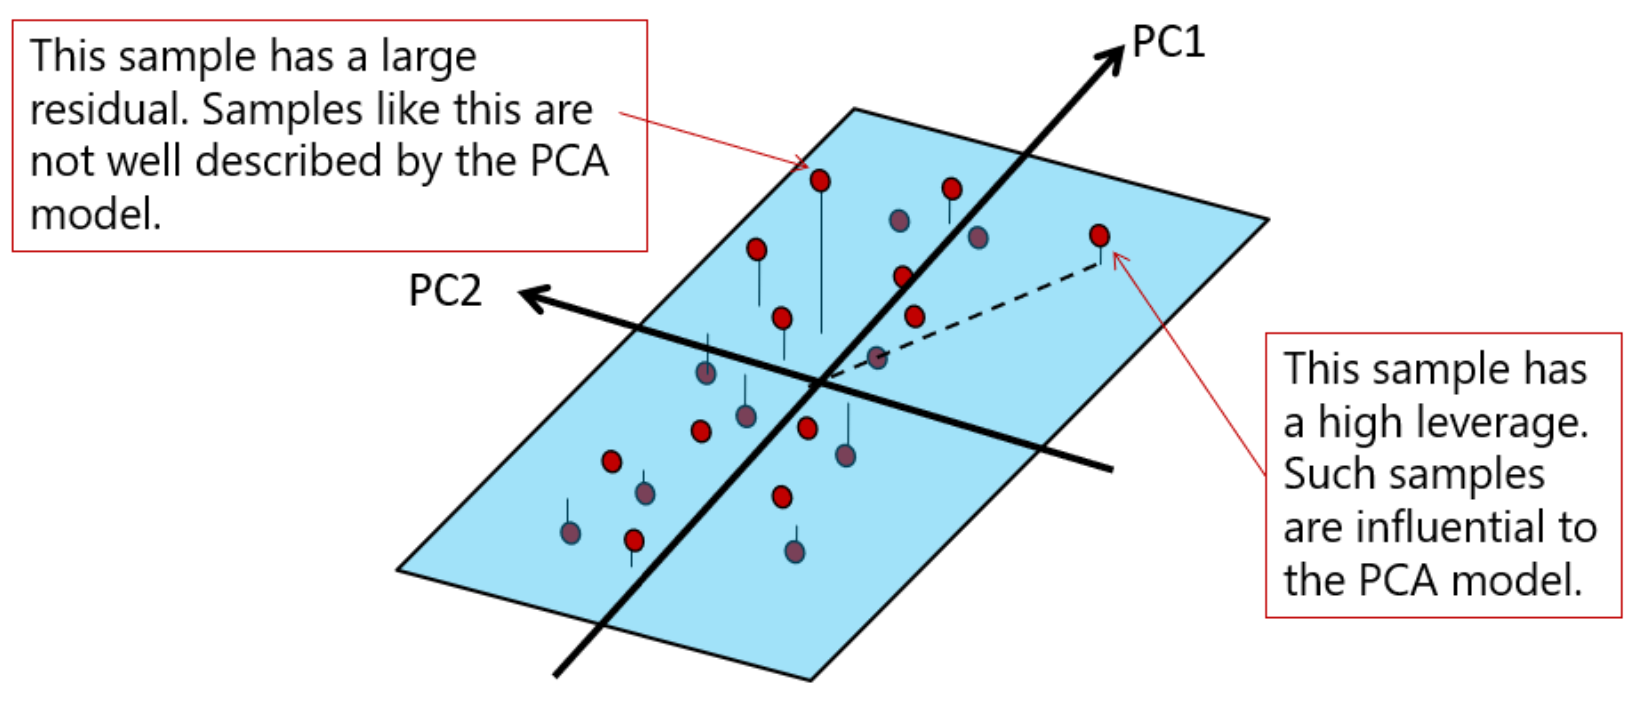
\includegraphics[width=0.8\textwidth]{figurer/utligger_illustrasjon.png}
	\caption{Ulike typer utliggere}
	\label{fig:utliggere}
\end{figure}

La $T$ være en matrise med scores slik at $X \approx T P^T$. Et mål på ``utliggerhet'' er bør da si noe om avstand til ``resten av dataen''. Noen slike verdier følger.

\subsubsection{Hotellings $T^2$}
\textbf{Hotellings} $T^2$ representerer avstanden til modellsenter i modellrommet (definert av $T$). For en observasjon $y_n$ er

\begin{equation}
	T_n^2 = \sum_{a=1}^A (t_{na} (T_a ^T T_a)^{-1} t_{na}^T) (n-1)
	\label{eq:hotelling_T2}
\end{equation}

$T^2$ er F-fordelt, og kan dermed brukes til å finne ut om $y_n$ kommer fra samme populasjon som resten av observasjonene (med et eller annet signifikansnivå). En typisk måte å visualisere dette på er som en ellipse i et score-plott. 

\subsubsection{Leverage}
For observasjonen $y_n$ er \textbf{leverage} gitt av

\begin{equation}
	h_n = \frac{1}{N} + t_{n, 1:A} (T_{1:A}^T T)^{-1} t_{n, 1:A}^T
\end{equation}
For leverage brukes vanligvis ikke signifikans for å bestemme kritisk grense (dvs. hva som defineres som en utligger), men heller en definisjon som er ganske så ad-hoc: $h_{\textrm{kritisk}} = \frac{3(A+1)}{N}$.

Summen av $h_n$ over alle $n$ observasjoner er 1, så leverage kan sees på som andelen varians en observasjon bidrar med. Denne verdien er lineært avhengig av Hotellings $T^2$ gjennom formelen

\begin{equation}
	T^2 = (N-1) (h - \frac{1}{N})
\end{equation}

\subsubsection{F- og Q-Residualer}
Som tidligere beskrevet er residualene for en modell $T P^T$ tilpasser $X$ gitt av

\begin{equation}
	E_A = X - \sum_{a = 1}^A t_a p_a^T
\end{equation}
der $A$ er antall PC-er brukt i modellen. For en enkelt observasjon $x_{nk}$ er residualen (gitt samme modell) gitt av

\begin{equation}
	e_{nk, A} = x_{nk} - \sum_{a = 1}^A t_{na} (p^T)_{ak}
\end{equation}

Disse gir ulike måter å representere residualene på. Om man er interessert i å undersøke enkeltobservasjoner (som gir mening siden utliggere jo er observasjoner) kan kritiske grenser for $e_{nk, A}$ estimeres vha. F- eller Q-fordelingen. 

\textbf{Q-residualen} er gitt av

\begin{equation}
	Q_{i, A} = e_{n, A}^T e_{n, A}
\end{equation}
og om man ønsker å finne kritisk Q-verdi for signifikans $\alpha$, kan man finne $c_\alpha$ i en tabell for standardnormalfordelingen, og bruke denne saftige formelen

\begin{equation}
Q_{a}=\theta_{1}\left(\frac{c_{a} \sqrt{2 \theta_{2} h_{0}^{2}}}{\theta_{1}}+\frac{\theta_{2} h_{0}\left(h_{0}-1\right)}{\theta_{1}^{2}}+1\right)^{\frac{1}{h_{0}}}
\end{equation}
der $\theta_1 = \textrm{trace}(E)$, $\theta_2 = \textrm{trace}(E^2)$, $\theta_3 = \textrm{trace}(E^3)$ og $h_0 = 1 - \frac{2 \theta_1 \theta_3}{3 \theta_2^2}$.

F-residualen kan finnes vha. Q-residualen, og regnes som mer konservativ. Den er gitt av

\begin{equation}
	F_{i, A} = \frac{Q_i}{K}
\end{equation}
Når man kjenner denne kan man gjennomføre en vanlig F-test.

Om man ikke vil bruke formler og finne disse verdiene manuelt, kan man bruke de innebygde metodene for dette som antageligvis allerede eksisterer i \texttt{verkøytet} man bruker for dataanalyse.


\subsection{Tidsserier}
Dette kapitlet er høyst relevant for alle som interesserer seg for dynamiske systemer.

\subsubsection{Modellstruktur}
Å jobbe med kontinuerlige systemer av ulineære differensiallikninger

\begin{equation}
	\dot{x} = f(x, u)
\end{equation}
har manger fordeler, men mulighet for å simulering og tilpassing av måledata er ikke en av dem. I den virkelige verden er vi typisk gitt tidsseriedata $X = [x_1 \quad \cdots \quad x_n]$, der hver $x_i$ er en kolonnevektor som inneholder en tidsserie med målinger av tilstanden $x_i$. Om vi mistenker at et system har en bestemt struktur $f(x, u)$ kan vi linearisere

\begin{equation}
	f(x) \approx f(x_0) + \nabla f_{x_0} (x - x_0)
\end{equation}

og deretter diskretisere

\begin{equation}
	\frac{df}{dt} \approx \frac{f(\Delta (k+1)) - f(\Delta k)}{\Delta}
\end{equation}

Vi innfører notasjonen $y(\Delta k) = y(k)$ for systemer i diskret tid, og z-operatoren

\begin{equation}
	z^r y(k) = y(k + r)
\end{equation}

Med denne operatoren definert er vi klar til å skrive alle differenslikninger

\begin{equation}
	y(t) + a_1 y(t-1) + \cdots + a_{n_a} y(t - n_a) = b_0 u(t) + \cdots + b_{n_b} u(t - n_b) + e(t)
\end{equation}

som en transferfunksjon

\begin{equation}
y(t) = \frac{B(q)}{A(q)} u(t) + \frac{1}{A(q)}e(t)
\end{equation}

der 

\begin{equation}
	A(q)=1+a_{1} q^{-1}+\ldots+a_{n_{a}} q^{-n_{a}}
\end{equation}

\begin{equation}
	B(q)=b_{1} q^{-1}+\ldots+b_{n_{b}} q^{-n_{b}}
\end{equation}

og vi av en eller annen grunn har byttet ut bokstaven $z$ med $q$. Denne modellen er en såkalt \textbf{ARX-modell}. AR fordi den er autoregressiv (y har en form for dynamikk), X fordi den er eksogen (har en input).

Om man kjenner $e$ kan man inkludere målinger av denne i modellen gjennom transferfunksjonen

\begin{equation}
	C(q)=1+c_{1} q^{-1}+\ldots+c_{n_{c}} q^{-n_{c}}
\end{equation}

og få en \textbf{ARMAX}-modell (MA = Moving Average) på formen

\begin{equation}
	y(t) = \frac{B(q)}{A(q)} u(t) + \frac{C(q)}{A(q)}e(t)
\end{equation}

Disse modellene har noen restriksjoner, f.eks. at både $u$ og $e$ har samme nevner (dvs. utsettes for samme dynamikk). En mer generell modell er \textbf{Box-Jenkins}-modellen, der

\begin{equation}
	y(t)=\frac{B(q)}{F(q)} u(t)+\frac{C(q)}{D(q)} e(t)
\end{equation}
om man setter $C(q) = D(q)$ for man en \textbf{Output Error}-modell. Det kan imidlertid være problematisk med så generelle modeller, så det er verdt å gjøre en vurdering av hvor komplisert modellstruktur man egentlig har behov for. 

\subsubsection{Ettstegsprediktorer}
Heretter vil vi anta at vi har gjort et valg av modellstruktur, og jobber med et system på formen

\begin{equation}
	y(t) = G(q) u(t) + H(q) e(t)
\end{equation}
hvor vi antar at $H(q)$ er monisk og minimum fase (dette blir nyttig senere).

Et naturlig ønske vil være å finne ut hvor systemet vil ende opp ved neste tidssteg gitt nåværende tilstand, dvs. finne en ettstegsprediktor $\hat{y}(t | t-1)$. Siden $u(t)$ velges av oss er den kjent, men $e(t)$ er ikke det. Derfor må effekten av denne estimeres. La $v(t) = H(q) e(t)$. Om vi klarer å finne en ettstegsprediktor $\hat{v}(t | t-1)$ kan vi enkelt finne $\hat{y}(t | t-1) = G(q) u(t) + \hat{v}(t | t-1)$. Men hvordan kan vi finne denne prediktoren? Jo, bare se her

\begin{equation}
v(t)=H(q) e(t)=\sum_{k=0}^{+\infty} h(k) e(t-k)=e(t)+\sum_{k=1}^{+\infty} h(k) e(t-k) \\
\end{equation}

\begin{equation}
\Longrightarrow \quad \widehat{v}(t | t-1)=\sum_{k=1}^{+\infty} h(k) e(t-k)
\end{equation}

fordi vi får et best mulig estimat ved å anta $e(t) = \mu_e = 0$, tror jeg. Skrevet om på transferfunksjonform får vi

\begin{equation}
	\hat{v}(t | t-1) = [H(q) - 1] e(t) = [1 - H^{-1}(q)] v(t)
\end{equation}
altså er det av interesse å finne $H^{-1}(q)$. Ved hjelp av litt utregning kan man da finne ut praktisk uttrykk for tilstandsprediktoren $\hat{y}$, gitt av

\begin{equation}
	\hat{y}(t | t-1) = H^{-1}(q) G(q) u(t) + [1 - H^{-1}(q)] y(t)
	\label{eq:predictor}
\end{equation}

Merk at siden vi antar $H(q)$ monisk, så inneholder leddet $[1 - H^{-1}(q)]$ ingen konstantledd, så prediktoren er ikke avhenig av kjennskap til $y(t)$. Vi har antatt $H(q)$ minimum fase, så impulsresponsen dens eksisterer og gir oss en veldefinert prediksjon. Nærmere bestemt er

\begin{equation}
	\left[H^{-1}(q) G(q)\right] u(t)=\left[\sum_{k=1}^{+\infty} \ell(k) q^{-k}\right] u(t)
\end{equation}

og

\begin{equation}
	\left[1-H^{-1}(q)\right] y(t)=\left[-\sum_{k=1}^{+\infty} \widetilde{h}(k) q^{-k}\right] y(t)
\end{equation}

I praksis vil vi lette på kravet om at summene skal gå til $\infty$, og heller la dem gå til $t$. Forhåpentligvis vil impulsresponsen avta raskt og eksponensielt nok til at prediksjonen blir nokså nærme sannheten.

Merk at hittil har vi ikke utnyttet noen informasjon om de statistiske egenskapene til $e(t)$. Det skal vi heller ikke gjøre, men en liten fun fact er at om $e(t)$ er Gaussisk, er den optimale $\hat{y}(t | t-1)$ gitt av Kalmanfilteret.

\subsubsection{Systemidentifikasjon}
Nå står vi bare igjen med et lite spørsmål: Hvordan finner vi $H^{-1}(q)$ og alle dens venner, som kreves for å gjennomføre disse prediksjonene? Dette gjøres ganske rett frem ved å minimere en eller annen loss-funksjon $\ell ( y - \hat{y} )$. Man velger da gjerne en mengde modellstrukturer $M_j$ med tilhørende parametre $\theta_j$ gitt av

\begin{equation}
	\theta_{j}^{*}=\underset{\theta_{j} \in \Theta_{j}}{\min } \sum_{t} \ell\left(-H^{-1}(q) G(q) u(t)+H^{-1}(q) y(t)\right)
	\label{eq:sysid}
\end{equation}
og velger modellstruktur basert på et eller annet kriterie (AIC, BIC, eller noe annet). Ved å sette inn verdiene for $H(q)$ og $G(q)$ gitt i avsnittet om modellstrukturer i likning \ref{eq:predictor}.

\subsubsection{Regularisering}
Denne problemformuleringen antar ingenting om systemet som identifiseres, men i praksis har vi gjerne ganske mye kunnskap om hvordan systemet oppfører seg (i hvert fall på et veldig grunnleggende nivå). For eksempel vil de fleste systemer av interesse ha en impulsrespons (og dermed også koeffisienter) som avtar eksponensielt. Denne kunnskapen kan tvinges på modellen i form av regularisering, og gjøres kanskje enklest ved å omformulere likning \ref{eq:sysid} til å være på matriseform og legge til et kvadratisk straffeledd. Dette illustreres best med et eksempel, hentet ganske direkte fra \cite{Chen2013}.

Se på en ARX-prosess

\begin{equation}
	y(t) = -a_1 y(t-1) - \cdots - a_n y(t-n) + b_1 u(t-1) + \cdots + b_m u(t-m)
	\label{eq:ARX}
\end{equation}
Denne kan skrives mer kompakt (som man gjerne gjør det når man f.eks. bedriver adaptiv regulering)

\begin{equation}
	y(t) = \varphi_y ^T (t) \theta_a + \varphi_u ^T (t) \theta_b = \varphi ^T (t) \theta
	\label{eq:ARX2}
\end{equation}
Vi er da interessert i å finne et estimat $\hat{\theta}$ som minimerer $\ell( y - \varphi ^T (t) \hat{\theta} )$. Regularisering introduseres da med en matrise $\Pi$, som har det navnet fordi den kan sees på som en Bayesisk prior til fordelingen til $\theta$ (som jeg så vidt nevnte i det forrige kapittelet om regularisering). En slik kovariansmatrise vil da typisk (for en ARX-modell) se ut som følger

\begin{equation}
	\Pi = \begin{bmatrix}
		\Pi^a & 0 \\
		0 & \Pi^b
	\end{bmatrix}
\end{equation}
der elementene $\Pi^a_{i, j} = C \min(\lambda^j, \lambda^k)$ er bestemt av parameterne $C$ og $\lambda$, og inkorporer kunnskapen om at impulsresponsen til systemet avtar eksponensielt (det samme gjelder for $\Pi^b$, potensielt med andre parameterverdier). Det endelige regresjonsproblemet blir da

\begin{equation}
	\hat{\theta} = \textrm{argmin}_\theta \; \ell (y - \varphi ^T (t) \theta) + \theta^T \Pi \theta
\end{equation}

\subsubsection{Annet}
Merk at det finnes massevis av praktiske hensyn som burde tas, som ikke er nevnt her. Et av de viktigste er persistent eksitasjon, som handler om hvor mye informasjon den gitte inputen gir om systemets dynamikk. For eksempel vil ikke et pådrag $u(t) = 0$ gi særlig mye informasjon om $G(q)$. Om $G(q)$ er komplisert vil $u(t)$ typisk også måtte være nokså komplisert for å få vite alt man trenger om $G(q)$. Et typisk krav for mange parameterestimeringsmetoder er at $u(t)$ må oppfylle at det eksisterer konstanter $\alpha_0, \alpha_1, T_0 > 0$ slik at 

\begin{equation}
	\alpha_0 I \leq \frac{1}{T_0} \int_t^{t + T_0} u(\tau) u(\tau)^T d\tau \leq \alpha_1 I \quad \textrm{for alle } t \leq 0
\end{equation}
$u(t)$ kalles da persistent eksiterende.



\newpage
\end{document}
